\chapter{Revisão teórica}



\section{Magnetismo}

Magnetismo é o fenômeno onde um material ou objeto causa uma força,
descrita como magnética, que repele ou atrai outros materiais e objetos susceptíveis. Este fenômeno é consequência de um movimento de cargas elétricas, algo que também surge em condutores elétricos de diversos tipos. Estas cargas em movimento são descritas em campos vetoriais, denominados campo magnético.\cite{callister2010}

A relação entre o campo magnético e o meio é representada pela equação \ref{eq:bcalc}, onde a intensidade de campo magnético é dada por H, cuja unidade é A/m; μ representa a permeabilidade magnética do meio em Henrys/m e, B representa a densidade de fluxo magnético, ou indução magnética, dado em T (Tesla). \cite{callister2010}

\begin{equation}
    B =\mu H
    \label{eq:bcalc}
\end{equation}

\section{Campo Magnético Uniforme}
Campo Magnético é a região ao redor de um imã, na qual ocorre um efeito magnético. Esse efeito é percebido pela ação de uma força magnética de atração ou de repulsão. O campo magnético pode ser definido pela medida da força que o campo exerce sobre o movimento das partículas de carga, tal como um elétron.\cite{mussoi2}

A representação visual do campo magnético é feita através de linhas de campo magnético, também conhecidas por linhas de indução magnética ou ainda por linhas de fluxo magnético, que são linhas envoltórias imaginárias. As linhas de campo magnético são linhas fechadas que saem do pólo norte e entram no pólo sul. \cite{mussoi2}

No caso de um imã em forma de ferradura, as linhas de campo entre as superfícies paralelas
dispõem-se praticamente paralelas, originando um campo magnético uniforme. No campo magnético
uniforme, todas as linhas de campo têm a mesma direção e sentido em qualquer ponto. Na figura \ref{fig:muss2} é mostrada essa situação. \cite{mussoi2}

\begin{figure}[H]
    \centering
     \caption{Linhas de campo uniforme e em imã permanente}
     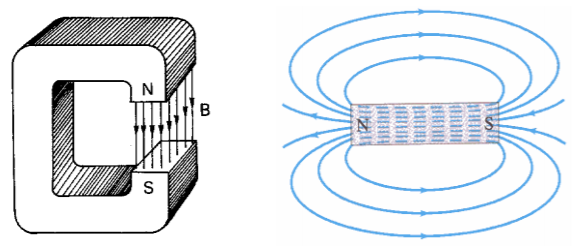
\includegraphics[width=0.8\textwidth]{./img/mussoi10.png}
     \caption*{Fonte: \cite{mussoi2}}
     \label{fig:muss2}
\end{figure}


\section{Campo Magnético gerado no centro de uma Espira Circular}
Um condutor em forma de espira circular quando percorrido por corrente elétrica é capaz de
concentrar as linhas de campo magnético no interior da espira, como mostrado na figura \ref{fig:campoc}. Isso significa que
a densidade de campo magnético resultante no interior da espira é maior que a produzida pela mesma
corrente no condutor retilíneo. \cite{mussoi1} 

\begin{figure}[H]
    \centering
     \caption{Campo magnético em uma espira circular}
     \subfloat[Linhas de campo magnético mostradas através de pó de ferro]{%
       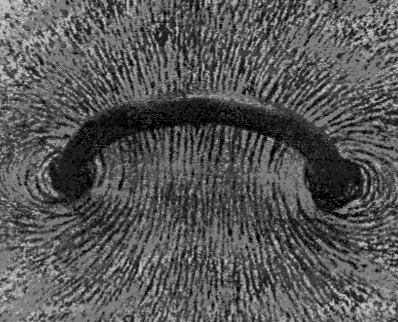
\includegraphics[width=0.45\textwidth]{./img/campoes.png}
     }
    % \hfill
     \subfloat[Esboço do campo vetorial magnético formado por uma espira]{%
      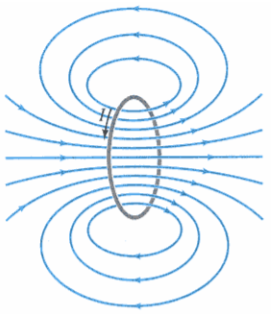
\includegraphics[width=0.33\textwidth]{./img/mussoi2.png}
     }
     \label{fig:campoc}
     \caption*{Fonte: \cite{mussoi1}}
\end{figure}

\section{Bobina de Helmholtz}
Segundo \cite[p. 11, 12, tradução nossa]{caldeira2017}:

\begin{quoting}[rightmargin=0cm,leftmargin=4cm]
{\footnotesize 
Inventado por Hermann von Helmholtz em meados do século XIX, a bobina de Helmholtz é um dispositivo que produz campos magnéticos quase uniformes. É composto por duas bobinas circulares que são posicionadas paralelamente umas às outras a uma distância igual ao raio de cada uma e que partilham o mesmo eixo central (ver figura \ref{fig:bh}). Este dispositivo produz um campo magnético composto por linhas paralelas no centro do aparelho quando a corrente flui dentro dos fios que compõem a bobina. A direção do campo magnético pode ser previsto usando a regra da mão direita e a intensidade do campo magnético é calculada no centro usando uma derivação da lei Biot-Savart:

\begin{equation}
    B = 	\left ( \frac{4}{5} \right )^{\frac{3}{2}}\cdot \frac{\mu 0 \cdot n \cdot I}{R} [T]
    \label{eq:helmholtzCoil}
\end{equation}


}
\end{quoting}

Na equação \ref{eq:helmholtzCoil}, B representa a indução magnética, $\mu$0 a permeabilidade magnética do vácuo, n o número de espiras, I a corrente elétrica que passa pela bobina e R o raio dos enrolamentos da bobina e também a distância entre os dois enrolamentos que compõe a bobina de Helmholtz, isto pode ser observado na figura \ref{fig:bh}.

\begin{figure}[H]
    \centering
     \caption{Bobina de Helmholtz.}
     \subfloat[Geometria da bobina]{%
       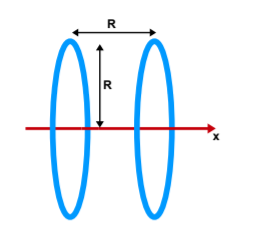
\includegraphics[width=0.3\textwidth]{./img/imagensExplicacoes/bobinaH.png}
     }
    % \hfill
     \subfloat[Esboço das linhas de campo]{%
      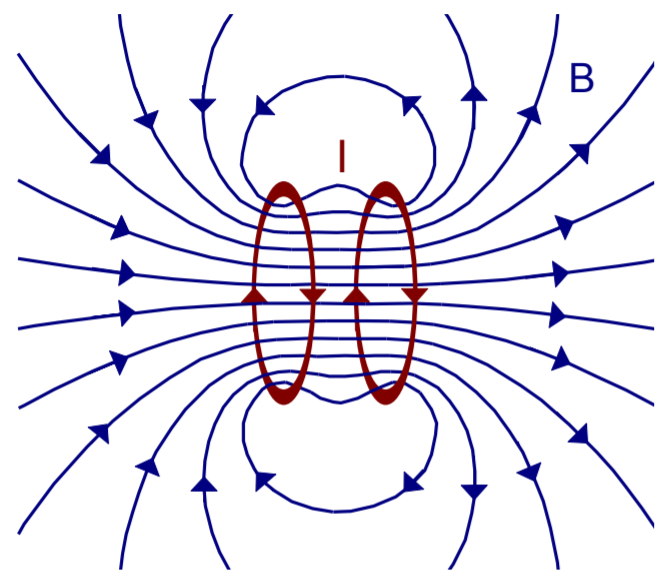
\includegraphics[width=0.3\textwidth]{./img/imagensExplicacoes/bobinaH2.png}
     }
     \label{fig:bh}
     \caption*{Fonte: \cite{caldeira2017}.}
\end{figure}

\subsection{Bobina de Helmholtz 3D}

Para um melhor entendimento do que seria uma bobina de Helmholtz 3D, na figura \ref{fig:bob3d} há uma ilustração de 3 bobinas de Helmholtz alinhadas de forma ortogonal, centradas no mesmo ponto, para gerar um campo homogêneo no centro da estrutura, cada par de enrolamentos paralelos é considerado uma bobina de Helmholtz e o conjunto dos 3 pares em direções ortogonais é a chamada bobina de Helmholtz 3D, que é capaz de gerar uma indução magnética em qualquer direção do espaço tridimensional, representado pela esfera no centro da estrutura.

\begin{figure}[H]
    \centering
     \caption{Ilustração das bobinas de Helmholtz.}
     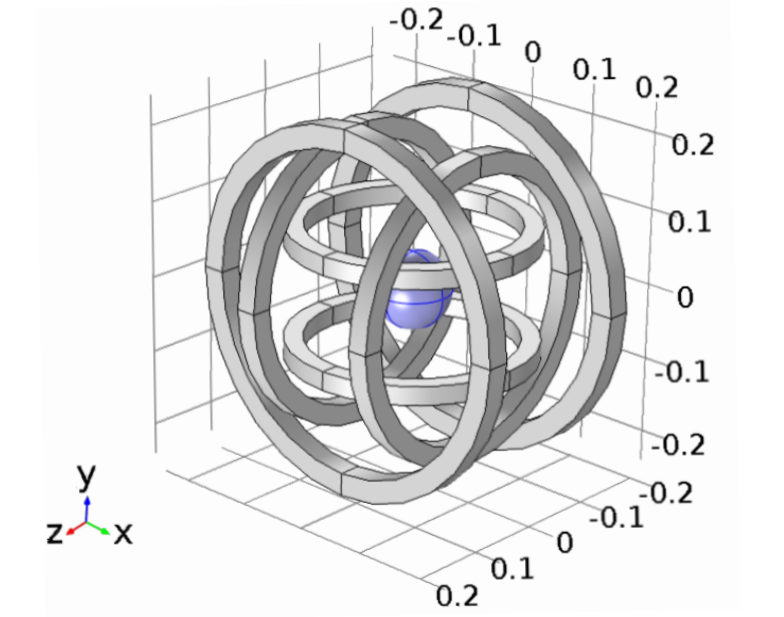
\includegraphics[width=0.65\textwidth]{./img/3dHMC.png}
     \caption*{Fonte: \cite{3dHelm}}
     \label{fig:bob3d}
\end{figure}

\section{Sensor magnético}

Um sensor magnético é um dispositivo capaz de detectar um campo magnético e transmitir as informações correspondentes. Portanto, um sensor magnético é um transdutor que converte um campo magnético em informação.\cite{popovic2003hall}

\section{Conversor de ponte completa (Ponte H)}
O conversor de ponte completa é um circuito utilizado para converter um sinal CC em um sinal CA, chaveando alternadamente entre chaves (S1 e S2 ou S3 e S4), como é demonstrado na figura \ref{fig:ponteh1}. Essa estrutura é também chamada de ponte H, se não houver chaveamento, pode-se apenas inverter a tensão da carga. \cite{hart2011power}

\begin{figure}[H]
    \centering
     \caption{Ponte H}
     \subfloat[Modelo do circuito]{%
       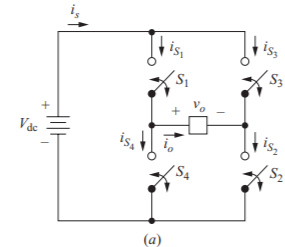
\includegraphics[width=0.5\textwidth]{./img/hart2.png}
     }
     \subfloat[Possibilidades de utilização]{%
       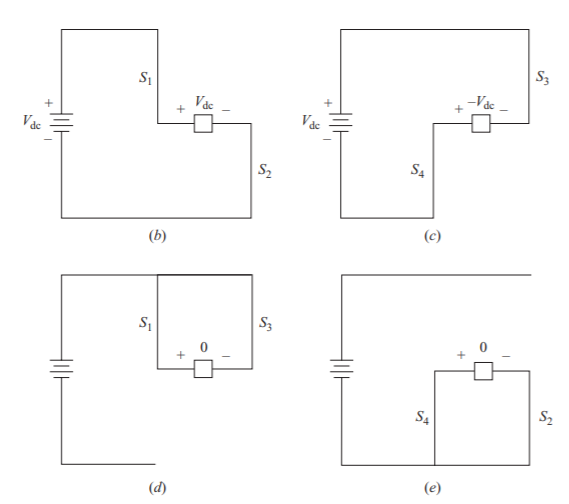
\includegraphics[width=0.5\textwidth]{./img/hart3.png}
     }
    % \hfill
     \caption*{Fonte:\cite{hart2011power}}\label{fig:ponteh1}
\end{figure}

Uma observação importante a comentar-se é que S1 e S4 não devem ser fechados ao mesmo tempo, nem S2 e S3 no caso da figura \ref{fig:ponteh1}. Caso contrário, existiria um curto-circuito através da fonte CC. \cite{hart2011power}

\section{Relação sinal ruído}

Um sinal, x(t), pode ser modelado como a soma do sinal desejado, s(t), e um sinal de ruído de faixa estreita, n(t), como mostrado na equação \ref{eq:sr}. \cite{haykinintrodução}

\begin{equation}
    \label{eq:sr}
    x(t) = s(t) + n(t)
\end{equation}

Os dois termos do lado direito da equação \ref{eq:sr} são aleatórios. O sinal é aleatório devido a imprevisibilidade de seu conteúdo de informação e o ruído é aleatório por natureza. Os dois parâmetros mais simples para descrever parcialmente uma variável aleatória são a média e a variância. Deslocamentos CC são considerados como sendo nulos. Consequentemente, para processos de média nula, uma simples medida da qualidade do sinal é a razão das variâncias dos sinais desejado e não desejado. Com esta base, a razão sinal/ruído é formalmente definida pela equação \ref{eq:sr2} \cite{haykinintrodução}

\begin{equation}
    \label{eq:sr2}
    SRN = \frac{E[s(t)^2]}{E[n(t)^2]}
\end{equation}

SRN é a relação sinal ruído e E é operador esperança. Para um sinal de comunicação, o nível do sinal quadrático é geralmente proporcional à potência. Consequentemente, a razão sinal/ruído é geralmente considerada como a relação da energia média do sinal por unidade de tempo pela energia média do ruído por unidade de tempo. \cite{haykinintrodução}
 
Segundo \cite{noiseRedArt}, para cada amostra de um sinal, se forem feitas N medidas, e a amostra for definida como a média dessas N medidas, a razão sinal ruído deste sinal é aumentada em $\sqrt{N}$. Isso é representado na equação \ref{eq:SRNn5}.

\begin{equation}
    \label{eq:SRNn5}
    SRN_N = \sqrt{N}\cdot SRN_1
\end{equation}

Neste caso a $SRN_1$ é representada pela razão entre o o sinal, s(kT), amostrado em períodos de tempo constante T e a variância do sinal $\sigma _n$ ou ruído RMS. Isso é mostrado na equação \ref{eq:as}. \cite{noiseRedArt}

\begin{equation}
    \label{eq:as}
    SRN_1 = \frac{s(kT)}{\sigma _n}
\end{equation}

\section{Python}
Nas palavras de \cite{bandeira2019}:
\begin{quoting}[rightmargin=0cm,leftmargin=4cm]
{\footnotesize 
Python é uma linguagem de programação de alto nível de abstração, utilizando o interpretador CPython como sua implementação padrão. Python é multiparadigma, encorajando o uso de programação orientada à objetos e de outros paradigmas para que o programador tenha a liberdade de decidir a maneira mais interessante de resolver diversos problemas. Introduzida em 1991 por Guido van Rossum,
Python possui uma gramática simples e poderosa.
}

\end{quoting}

\subsection{magPyLib}

É um pacote livre em Python para o cálculo de campos magnéticos, correntes e momentos magnéticos. Os campos magnéticos são determinados através de soluções analíticas as quais resultam em um tempo de computação muito mais rápido que soluções que empregam elementos finitos. \cite{magpy2020} 

\subsection{pySerial}

É uma biblioteca de código aberto que abstrai o acesso à porta COM virtual para o uso em computadores, empregado na programação \textit{python}, ou seja, da ao usuário o acesso a porta serial através de funções sem que o usuário tenha que se preocupar com o hardware da sua maquina. \cite{pySerial}

\subsection{pyVisa}

VISA é um acrônimo para \textit{Virtual Instrument Software Architecture}. VISA é uma API (\textit{Application Programming Interface}) de comunicação padrão da indústria de teste e medição para uso com dispositivos de teste e medição. Algumas vezes chamado de \textit{driver} de comunicação. VISA permite o desenvolvimento de programas independentemente do barramento de dados utilizado pelo instrumento. O uso de bibliotecas VISA permite a comunicação para muitas interfaces, como USB (\textit{Universal Serial Bus}) e Ethernet.\cite{visaRef}

A especificação VISA tem ligações explícitas com Visual Basic, C e G (linguagem gráfica do LabVIEW). Python pode ser usado para chamar funções de uma biblioteca compartilhada VISA (.dll, .so, .dylib) permitindo o desenvolvimento de diversas aplicações. Além disso, Python pode ser usado para acessar diretamente a maioria dos barramentos de dados usados por instrumentos, e é por isso que se pode prever a implementação do padrão VISA diretamente em Python. PyVISA é um \textit{wrapper} Python para bibliotecas compartilhadas VISA.\cite{pyvisaRef}
